\documentclass{article}
\usepackage[T1]{fontenc}
\usepackage{lmodern}
\usepackage{graphicx}
\usepackage{amsmath,amssymb}
\usepackage[a4paper,margin=2cm]{geometry}
\usepackage[absolute,overlay]{textpos}
\setlength{\TPHorizModule}{1mm}
\setlength{\TPVertModule}{1mm}
\usepackage[indonesian]{babel}
\usepackage{hyperref}
\setlength{\emergencystretch}{2em}
% unit: Halaman 96

\begin{document}

% === Halaman 96 (llm) ===

\section*{Lester S. Hill}

\vspace{198.99mm}

From Wikipedia, the free encyclopedia

\textbf{Lester S. Hill} (1891--1961) was an American mathematician and educator who was interested in applications of mathematics to communications. He received a bachelor's degree (1911) and a master's degree (1913) from Columbia College and a Ph.D. from Yale University (1926). He taught at the University of Montana, Princeton University, the University of Maine, Yale University, and Hunter College. Among his notable contributions was the Hill cipher. He also developed methods for detecting errors in telegraphed code numbers and wrote two books.

\vspace{20mm}

\subsection*{References}

\begin{enumerate}
    \item $\wedge$ Christensen, Chris (2014). "Lester Hill Revisited". \textit{Cryptologia}. 38 (4): 300--301. doi:10.1080/01611194.2014.915260. S2CID 45603857. Retrieved November 9, 2018 -- via ResearchGate.
    \item $\wedge$ a b "Dr. Lester S. Hill", \textit{Chicago Tribune}, January 10, 1961. p. 10. "Dr. Lester S. Hill, 70, mathematician and cryptographer, died today in Lawrence hospital after a long illness. Hill was commended for application, of higher mathematics to the construction of secret codes."
\end{enumerate}

% deskripsi: Infobox Wikipedia mengenai profil Dr. Lester S. Hill yang berisi foto, tanggal lahir, tanggal wafat, pekerjaan, dan karya terkenal.
% bbox normalisasi: [0.5700, 0.2200, 0.8200, 0.8900]
\begin{textblock*}{52.50mm}(119.70mm,65.34mm)
\noindent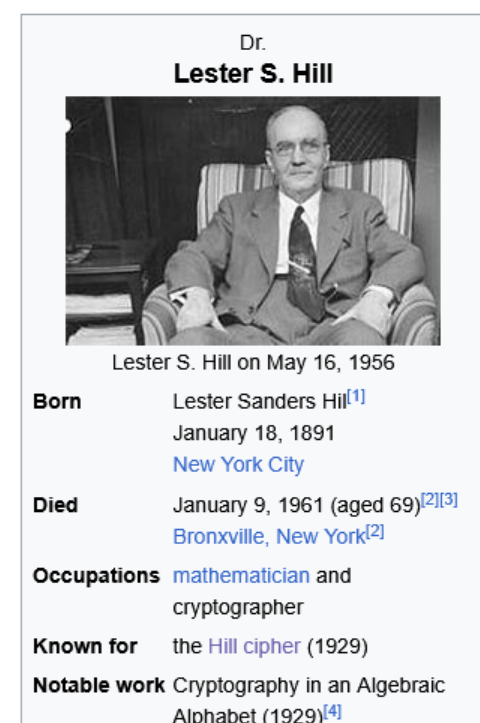
\includegraphics[width=52.50mm,height=198.99mm]{../../images/llm/page_096_img_01.png}%
\end{textblock*}

\end{document}
